%----------------------------------------------------------------------------
\chapter{The core software}\label{chap:Core software}
%----------------------------------------------------------------------------
%Glossary entries
\newglossaryentry{utc}{name=UTC, description={Coordinated Universal Time}}
\newglossaryentry{pqr}{name=PQR, description={Coordinated Universal Time}}
%----------------------------------------------------------------------------
This chapter presents the structure and operation of the core software system of the Traffic Sensor, in particular with regard to the effective image processing algorithms and software development paradigms that facilitate the real-time operation of the system.

The core software is responsible for the processing of the video stream itself.
It identifies the vehicles, classifies them and estimates parameters, including speed and following distance.
 
Besides that, the software supports other supplementary features, like the evaluation of the system's precision, and correction of the calibration rectangle.
Although these features are implemented architecturally in the same software unit, the supplementary elements are discussed in section \ref{sec:SupplementarySoftware}, since they do not strictly belong to the core of the Traffic Sensor.
%----------------------------------------------------------------------------
\section{Software architecture}\label{sec:software_architecture}
%----------------------------------------------------------------------------
In this section the architectural structure of the framework, including the data storage technique, the processing method and the parallel operation of the system are discussed.

\begin{figure}[!h]
	\centering
	\includesvg[width=0.8\textwidth,pretex=\Large]{arbiter_pipeline.pdf_tex}
	\caption[The structure of the core software architecture]{The function and operation of the Arbiter, Processors and the Media Store. The Processors that implement a unified interface are controlled by the Arbiter. There are an arbitrary number of Processors in the system, each of them can be exchanged, deleted, and the sequence of processors can be expanded with new functions as well, thus realizing a plug-in architecture. Although each Processor can manage a single Frame or Timeline Image column at once, since they operate simultaneously on their threads, a large amount of data is processed at the same time. The data resources of the system are accessed through the Media Store protected by mutexes.\label{fig:arbiter_pipeline}}
\end{figure}

\subsection{Plug-in architecture, Processors}
Since the Traffic Sensor software ought to meet several requirements, like real-time operation in a resource-limited environment, it is necessary that the software exploits the target hardware as far as possible.
Moreover, because the framework is a conceptional prototype, the possibility of further improvement of features -- especially the implementation of additional processing steps -- is important.

To satisfy these specifications, a plug-in architecture was implemented.
Each of the processing steps are executed by its own software component, called a Processor.
The execution is controlled by a central unit, the Arbiter.
The Processors have a unified interface, through which they communicate with the Arbiter.
The Arbiter can control an arbitrary number of Processors, and thanks to their unified interface, each of them can be deleted or replaced with a different implementation, and if needed, further steps can be integrated into the system as well.

\subsection{Parallel processing}
To utilize the hardware and for the sake of real-time processing, Processors operate simultaneously in a pipeline-like manner as depicted in figure \ref{fig:arbiter_pipeline}.
For process synchronization are thread-pool is used, where every Processor owns a thread, and the Arbiter controls their work-flow.
Thanks to this, although each unit can only process a single Frame and Timeline Image column at once, the system can manage 10--15 columns and images at the same time, depending on the number of Processors.

\subsection{Media storage}
The Processors reach the required Frames and columns through the Media Store unit.
The Media Store contains the system's resources in the form of Timeline Images and Frame-strips.
Since the memory of the embedded hardware is very limited, only a finite amount of data can be cached.
To achieve this, after detection and data extraction are finished, the henceforward unused Timeline Images and Frame Strips are discarded.
To attain a continuous operation with a constant memory usage, approximately 20--30 Frames in a Frame-strip and 500 columns in a Timeline Image are usually stored.
For further changes and improvements, the maximum number of saved units can be specified through the system's configuration files (detailed in section \ref{subs:ProjectConfigurator}).
To prevent deadlocks, the resources are accessed through mutexes.

The specific Timeline Images and Frame-strips used by the Traffic Sensor are detailed as follows.

\subsubsection{Frame-strips}
Each of the Frame-strips store the successive frames of the video stream, either in its raw form, or transformed.
\begin{enumerate}
	\item \textbf{Raw Frame-strip:} The Raw Frame-strip is the sequence of images directly recorded by the camera. (Figure \ref{fig:raw_frame})
	
	\item \textbf{Original Frame-strip:} The Original Frames are transformed versions of the Raw Frames. The transformation creates a standard frame format that is independent of the Raw Frames' size or the specific traffic scene, and that supports effective processing. (Figure \ref{fig:original_frame})
	
	\item \textbf{MOG2 Frame-strip:} The MOG2 Frame-strip is a sequence of the result images of the MOG2 background-subtraction algorithm, the MOG2 Frames. MOG2 Frames are one-channel, binary images, with foreground objects labelled with the value 255 (white), and background labelled with 0 (black). The Foreground objects of the MOG2 Frames are blobs. (Figure \ref{fig:mog2_frame})
\end{enumerate}

\subsubsection{Timeline Images}
The Timeline images can either be extracted from the Frame-strips (Original Timeline or MOG2 Timeline) or created from the latter calculated data (Motionless Timeline, Parameter Timelines).

\begin{enumerate}
	\item \textbf{Original Timeline:} The Original Timeline is a three-channel, color image, extracted from the Original Frame-strip, by stacking the states of the tripwire of the Original Frame. (Figure \ref{fig:original_timeline})
	
	\item \textbf{MOG2 Timeline:} The MOG2 Timeline derives from the MOG2 Frame, thus it is a one-channel, binary image, where foreground objects are labelled with the value 255 (white), and background is labelled with 0 (black). The foreground objects of the MOG2 Timeline are called timeline-blobs later identified as vehicles. (Figure \ref{fig:mog2_timeline})
	
	\item \textbf{Motionless Timeline:} Motionless Timeline stores the data of stopped vehicle in the form of a one-channel image. (Figure \ref{fig:motionless_timeline})
	
	\item \textbf{Size, Speed, Following Distance Timeline: Parameter Timelines:}
	The Parameter Timelines store the estimated data of the vehicles, including their speed, length and following distance. All of the above data are extracted using the MOG2 Frame-strip, by measuring the size, speed and distance of the objects that occupy or enclose the tripwire at a specific time.
	To limit memory usage, the data is stored in the form of one-channel matrices of signed (for speed that has a direction) or unsigned integers. For human understanding the data is transformed and represented as color and grayscale images. (Figures \ref{fig:size_timeline}--\ref{fig:fd_timeline})
\end{enumerate}

\begin{figure}[!h]
	\centering
	\begin{subfigure}[!h]{0.5\textwidth}
		\includegraphics[width=\textwidth]{raw_frame.png}
		\caption{Raw Frame. \label{fig:raw_frame}}
	\end{subfigure}
	\quad
	\begin{subfigure}[!h]{0.35\textwidth}
		\includegraphics[width=\textwidth]{original_frame.png}
		\caption{Original Frame.\label{fig:original_frame}}
	\end{subfigure}
	\hfill
	\begin{subfigure}[!h]{0.35\textwidth}
		\includegraphics[width=\textwidth]{mog2_frame.png}
		\caption{MOG2 Frame. \label{fig:mog2_frame}}
	\end{subfigure}
	\caption[Frame-strip types]{Frames representing each type of Frame-strips used by the Traffic Sensor system.\label{fig:frame_types}}
\end{figure}

\begin{figure}[!h]
	\centering
	\begin{subfigure}[!h]{0.9\textwidth}
		\includegraphics[width=\textwidth]{Original.png}
		\caption{Original Timeline.\label{fig:original_timeline}}
	\end{subfigure}
	\hfill
	\begin{subfigure}[!h]{0.9\textwidth}
		\includegraphics[width=\textwidth]{Mog2_tl.png}
		\caption{MOG2 Timeline.\label{fig:mog2_timeline}}
	\end{subfigure}
	\hfill
	\begin{subfigure}[!h]{0.9\textwidth}
		\includegraphics[width=\textwidth]{Motionless.png}
		\caption{Motionless Timeline. \label{fig:motionless_timeline}}
	\end{subfigure}
	\hfill
	\begin{subfigure}[!h]{0.9\textwidth}
		\includegraphics[width=\textwidth]{Size.png}
		\caption{Size Timeline. \label{fig:size_timeline}}
	\end{subfigure}
	\hfill
	\begin{subfigure}[!h]{0.9\textwidth}
		\includegraphics[width=\textwidth]{Speed.png}
		\caption{Speed Timeline. \label{fig:speed_timeline}}
	\end{subfigure}
	\hfill
	\begin{subfigure}[!h]{0.9\textwidth}
		\includegraphics[width=\textwidth]{Following_distance.png}
		\caption{Following Distance Timeline. \label{fig:fd_timeline}}
	\end{subfigure}
	\caption[Timeline image types]{The representation of Timeline Image types used by the Traffic Sensor system for data storage.\label{fig:timeline_types}}
\end{figure}

\section{Processing steps}\label{sec:processing_steps}
%----------------------------------------------------------------------------
The processing of the video-stream consists of four main stages, as depicted in figure \ref{fig:processing_steps}.

%\clearpage
%\addtolength{\voffset}{-.3in}
\begin{figure}[p]
	\thispagestyle{empty}
	\centering
	\thisfloatpagestyle{empty}
	\vspace*{-.3in}
	%\includesvg[width=\textwidth]{full_system_flowchart}
	\includegraphics[width=\textwidth]{full_system_flowchart.png}
	\caption[Video processing steps]{Steps of the processing of the video stream in the core software of the Traffic Sensor.\label{fig:processing_steps}}
\end{figure}

%\FloatBarrier
%\addtolength{\voffset}{+.3in}

The first step is preprocessing, that is the remapping of each frame to achieve a standard form for effective processing.
Second, a background-subtraction and its post-corrections are applied to detect the moving vehicles precisely.
The third stage is data extraction, including vehicle detection, classification and parameter calculation.

The final step is system evaluation and testing. 
Since this step is optional, and is only available when the system is tested during development, when the operation is not continuous, it is considered a supplementary software element, and is discussed in detail in section \ref{sec:SupplementarySoftware}.
%----------------------------------------------------------------------------
\subsection{Preprocessing}\label{sec:preprocessing}
%----------------------------------------------------------------------------
In the preprocessing stage a series of transforms are performed on each Raw Frame as seen in figure \ref{fig:transforms}.
As a result of remapping, a standard frame-scheme is created, that is independent of the video file format, camera type, placement and the sensor's environment.
This regular form has a pre-defined size, that is small enough to be processed in real-time, and is simple enough to be rapidly searched and measured.
The result of the remapping of the Raw Frame is an Original Frame, from which a column is extracted and added to the Original Timeline.

The first stage is perspective compensation.
At this point, the image, distorted by perspective transform, is remapped based on a calibration rectangle, so that lengths in the frame become independent from the distance of the camera.
The following vehicle-size calculation and classification strongly relies on the assumption that vehicle-lengths are not subject to perspective distortion, and are irrelative to their position in the frame.
The calibration rectangle is defined manually using the Project Configurator user interface (UI), that is detailed in section \ref{subs:ProjectConfigurator}.

The second stage is rotation of the frame, so that the tripwire becomes vertical.
As a result of the vertical tripwire, it is possible to measure in the dimension perpendicular to the tripwire simply by reading certain rows of the image.
This method, considering the image-storage technique of the OpenCV library, where frames are stored as an array of rows in the memory, speeds up the computation significantly, and simplifies searching in frames.

In the third level of preprocessing a frames are resized in order to decrease the number of pixels and the computation time, and increase the speed of processing.
The end-size of the frame can be specified through the configuration files, and is usually 320 by 240 pixels.

\begin{figure}[!h]
	\centering
	%\includesvg[clean,width=\textwidth,pretex=\relsize{2}]{frame_transforms}
	\includegraphics[width=\textwidth]{frame_transforms.png}
	\caption[Steps of the preprocessing stage]{Preprocessing steps: the transformations performed on each frame before the background-subtraction and detection phase. The goal is to create an effective frame format for the following processing steps.\label{fig:transforms}}
\end{figure}
%----------------------------------------------------------------------------
\subsection{Background-subtraction}\label{sec:background-subtraction}
%----------------------------------------------------------------------------
The second phase of processing is background-subtraction, that is the separation of moving objects form the static background in each frame.
This step creates the MOG2 Frame and Timeline as a result of background-subtraction.
The correction of the subtraction method use the Motionless Timeline.

The background is labelled using a GMM-based method, Mixture of Gaussians 2 (MOG2), that is available in the OpenCV library.
This method associates every pixel with a mixture of Gaussian intensity-distributions, and identifies each new data as background, if it is part of the constructed distribution-model, or as a moving object, if it falls out of the model's range.

The drawback of this technique is its complexity, that results in an increased computational cost and time.
Throughout the processing, background-subtraction is the most time-consuming of all of the outlined processing steps.
However, since the following steps rely on the accuracy of the result of the background-subtraction, the robustness and precision of the approach are essential.

Another drawback of background-modelling is that temporarily stopped objects that have been motionless for a while are missed, as they are being included into the background model.
The errors caused by this is corrected later on, by detecting immobile vehicles.

Although some approaches model only the tripwire's pixels as background--foreground, in our method background-subtraction takes place on the whole frame.
That is, because features, such as size and velocity are calculated by measuring objects' lengths in the MOG2 Frame, as further detailed in section \ref{chap:parameter_evaluation}.
After the background-subtraction, the result is corrected, in order to filter errors of the MOG2 output.

First, morphological opening followed by closing removes punctual noises, and smooths object contours in the MOG2 Frame.
As a result, the MOG2 Timeline is created.
After, stopped vehicles are detected, and saved to the Motionless Timeline.
As sudden light changes can cause an overreaction of MOG2, to prevent this, the MOG2 Frames are filtered.
If the count of a frame's white pixels exceeds a limit, the frame is cleared, and switched to background, to avoid false detections.
Although this process causes some vehicles to be missed, empirical analysis shows, that error rate is reasonably lower if the overreaction frames are filtered.
%----------------------------------------------------------------------------
\subsection{Data extraction}
%----------------------------------------------------------------------------
The required data is extracted after the MOG2 Timeline and Frame are created, and pixels of moving objects are identified.
First, timeline-blobs are selected with connected component analysis on the MOG2 Timeline image.

Afterwards the detection results are revised and corrected.
Some errors occur, because vehicles can fuse in the TI, if they cross the tripwire together. These merged objects are split based on their shapes, and saved as vehicles.

Also, errors may occur because of stopping vehicles, since their blobs slowly disappear and reappear in the MOG2 timeline.
Thus these vehicles have two separate blobs.
The split timeline-blobs are identified and recombined using the data of the Motionless Timeline. 

\begin{figure}[p]
	\centering
	\thisfloatpagestyle{plainlower}
	\includesvg[clean,width=\textwidth,pretex=\relsize{0.8}]{speed_size_following_distance}
	%\includegraphics[width=\textwidth]{speed_size_following_distance.png}
	\caption[The method for parameter calculation]{The basic idea of parameter calculation. Each feature is estimated with measuring lengths perpendicular to the Tripwire.\label{fig:size_speed_following_distance}}
\end{figure}

After the vehicle detection, parameters are evaluated and stored as timeline images.
The following section discusses the estimation of these parameters.

\subsubsection{Parameter evaluation}\label{chap:parameter_evaluation}
The next phase of data extraction is parameter calculation.
At this point, the length, speed and following distance of the identified vehicles are estimated and stored in the form of a timeline image.
The length, speed and distance of the vehicles are measured in the MOG2 Frames, and projected back to the Parameter Timelines.
The notation used in this section are explained in figure \ref{fig:parameter_notations}.

\begin{figure}[!h]
	\centering
	\includesvg[width=0.73\textwidth,pretex=\relsize{1.5}]{speed_size_notations}
	%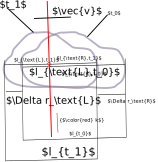
\includegraphics[width=0.73\textwidth]{speed_size_notations.png}
	\caption[The visualzation of the notations of parameter calculation]{Notations used in section \ref{chap:parameter_evaluation}. \label{fig:parameter_notations}}
\end{figure}

At each point in the Size Timeline the intensity value is calculated as follows:

\begin{displaymath}
 	\boldsymbol{TI_{\text{Size}}}(t,k) = 
	\begin{cases}
	l_{\text{L},t} + l_{\text{R},t}        & \quad \text{if } \boldsymbol{F_{\text{MOG2},t}} \text{ in the } k\text{th} \text{ point of the tripwire is occupied}\\
  	0		& \quad \text{if } \boldsymbol{F_{\text{MOG2},t}} \text{ in the } k\text{th} \text{ point of the tripwire is empty,}\\
	\end{cases}
\end{displaymath}

with $l_{\text{L},t}$, $l_{\text{R},t}$ being the perpendicular length of the left and right side of the object that occupies the tripwire.
The lengths are measured in pixels.

The intensities of the Speed Timeline are calculated with the lengths measured in 2 successive frames, as follows:

\begin{displaymath}
\boldsymbol{TI_{\text{Speed}}}(t_0,k) = 
\begin{cases}
\frac{\Delta r_{\text{L}} + \Delta r_{\text{R}}}{2}      & \quad \text{if } \boldsymbol{F_{\text{MOG2},t_0}} \text{ and } \boldsymbol{F_{\text{MOG2},t_1}} \text{ in the } k\text{th} \text{ point of} \\ & \quad \text{the tripwire are occupied}\\
0		& \quad \text{otherwise,}\\
\end{cases}
\end{displaymath}
 
where $\Delta r_{\text{L}}$ and $\Delta r_{\text{R}}$ are the displacements of the left and right edge of the object, that occupies the tripwire.
The vehicle lengths stored in the Size Time are later used for classification purposes.

The displacements are calculated with the left and right sides' lengths as follows:
\begin{gather*}
\Delta r_{\text{L}} = \left( l_{\text{L},t_0} - l_{\text{L},t_1} \right),  \\
\Delta r_{\text{R}} = \left( l_{\text{R},t_1} - l_{\text{R},t_0}\right).
\end{gather*}

The intensity values of the Following Distance (FD) Timeline are calculated as follows:

\begin{displaymath}
\boldsymbol{TI_{\text{FD}}}(t,k) = 
\begin{cases}
d_{\text{L},t} + d_{\text{R},t} 		& \quad \text{if } \boldsymbol{F_{\text{MOG2},t}} \text{ in the } k\text{th} \text{ point of the tripwire is empty,} \\ & \quad \text{and objects are detected on each side of the } k \text{th point}\\
0		& \quad \text{otherwise},
\end{cases}
\end{displaymath}

with $d_{\text{L},t}$ and $d_{\text{R},t}$ being the left and right side distances of the nearest objects.
The distances are estimated by counting the empty pixels on each side of the tripwire.

The calculated parameters are then either transferred in a raw form through the EnTalk\textsuperscript{TM} Network in the form of a report file (like following distance values, as detailed in section \ref{sec:reporting}), or used for classification purposes (like size values).
Although the speed measures are currently unused, possible future applications include the identification of road lanes, congestion detection, or the correction of Timeline Blobs of stopped vehicles.

\subsubsection{Classification}\label{sec:classification}
%----------------------------------------------------------------------------
The classifier of the Traffic Sensor is a computationally cheap and a rather less resource-intensive algorithm.

The vehicles are categorized based on one feature, their estimated length, that are computed using the Size Timeline.

Length was chosen as the primary feature of the classification, because under the aforementioned conditions, including the camera position, it is the most robust and discriminative feature.
Vehicle length is independent from the angle of the focal axis, and unlike width, it can be measured from the side of the road without being distorted.
This feature is also less noise-sensitive than other simple features, like intensity and color, since it is not affected by light-changes during the day.

\begin{figure}[!h]
	\centering
	%\includesvg[width=0.9\textwidth]{classification}
	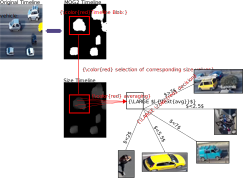
\includegraphics[width=0.9\textwidth]{classification.png}
	\caption[The classifier's operation]{The classification process. Each vehicle's length is estimated based on the corresponding size data, then categorized with a hard-decision classifier into four separate categories. \label{fig:classification}}
\end{figure}

To estimate their length $l_{\text{vehicle}}$, each vehicle's Timeline Blob (the blob region is denoted by $TB$) is projected to the Size Timeline, and the values corresponding to the blob's region are averaged, as depicted in figure \ref{fig:classification}. 
The length-feature is calculated using the following equation:

\begin{displaymath}
	l_{vehicle} = \frac{\mathlarger{\mathlarger{\sum}}\limits_{\substack{(x,y) \in \text{TB} \\ \boldsymbol{TI_{\text{Size}}}(x,y)\neq 0}} \boldsymbol{TI_{\text{Size}}}(x,y)}{n_{\text{NZpoints}}},
\end{displaymath}

with $n_{\text{NZpoints}}$ being the number of non-zero points in the Size Timeline.

\begin{table}[!h]
	\centering
	\begin{tabular}{ll}
		\toprule
		\textbf{Class} & \textbf{Length (m)} \\
		\midrule
		Pedestrian     & $< 2$               \\
		Cyclist        & $< 2.5$             \\
		Car            & $< 5.5$             \\
		Truck          & $< 7$               \\
		Other          & $ \geq 7$    \\
		\bottomrule          
	\end{tabular}
\caption{The five categories of the classification and their length-intervals.}
\label{tab:intervals}
\end{table}

The vehicles then categorized by a hard-decision classifier into five categories (figure \ref{fig:types}) .
The types were configured for common urban traffic scenes, thus they represent the most typical road user categories.
Since the classification data is used for emission estimation of greenhouse gases as well, the vehicle categories consist of vehicles with similar greenhouse emission profiles.
Although the class of cyclists and motorcycles is not homogeneous concerning their emission, this anomaly influences the estimation very moderately.
The "other" class represents vehicles with significant emission, including buses and lorries. 

The intervals of the categories were determined empirically and are noted in table \ref{tab:intervals}.

The sizes in the Size Timeline are converted to metrics with a scaling-factor that is calculated based on the size of the calibration rectangle's sides.

\begin{figure}[!h]
	\centering
	\begin{adjustbox}{minipage=\textwidth,scale=0.95}
	\centering
	\begin{subfigure}[b]{0.22\textwidth}
	\includegraphics[width=\textwidth]{cars.png}
	\caption{Cars.}
	\end{subfigure}
	\quad%
	\begin{subfigure}[b]{0.22\textwidth}
		\includegraphics[width=\textwidth]{trucks.png}
	\caption{Trucks.}
	\end{subfigure}
	\quad%
	\begin{subfigure}[b]{0.22\textwidth}
		\includegraphics[width=\textwidth]{bicicle.png}
	\caption{Bicycles.}
	\end{subfigure}
	\quad%
	\begin{subfigure}[b]{0.22\textwidth}
		\includegraphics[width=\textwidth]{ped.png}
	\caption{Pedestrians.}
	\end{subfigure}
	\quad
	\begin{subfigure}[b]{0.4\textwidth}
		\includegraphics[width=\textwidth]{other.png}
	\caption{Other.}
	\end{subfigure}

	\caption[Particular vehicle appearances for each category]{Some particular vehicle appearances that represent the system's classification categories.\label{fig:types}}
    \end{adjustbox}
\end{figure}
%----------------------------------------------------------------------------



